% =====================================================
% CHAPITRE 1 : ARCHITECTURE ET DÉPLOIEMENT
% =====================================================
\chapter{Architecture et Déploiement de l'Application E-commerce}

\section{Vue d'ensemble de l'architecture}

Notre système est une plateforme e-commerce construite selon une architecture microservices. Cette architecture a été spécifiquement conçue pour servir de cible aux expérimentations de chaos engineering, en exposant les vulnérabilités typiques des systèmes distribués : points de défaillance uniques, dépendances inter-services, et problématiques réseau.

\subsection{Architecture globale}

L'architecture se compose de cinq microservices métiers indépendants, orchestrés par une API Gateway et partageant une base de données PostgreSQL commune. Tous les composants sont conteneurisés avec Docker et communiquent via un réseau bridge isolé.

\begin{figure}[H]
\centering
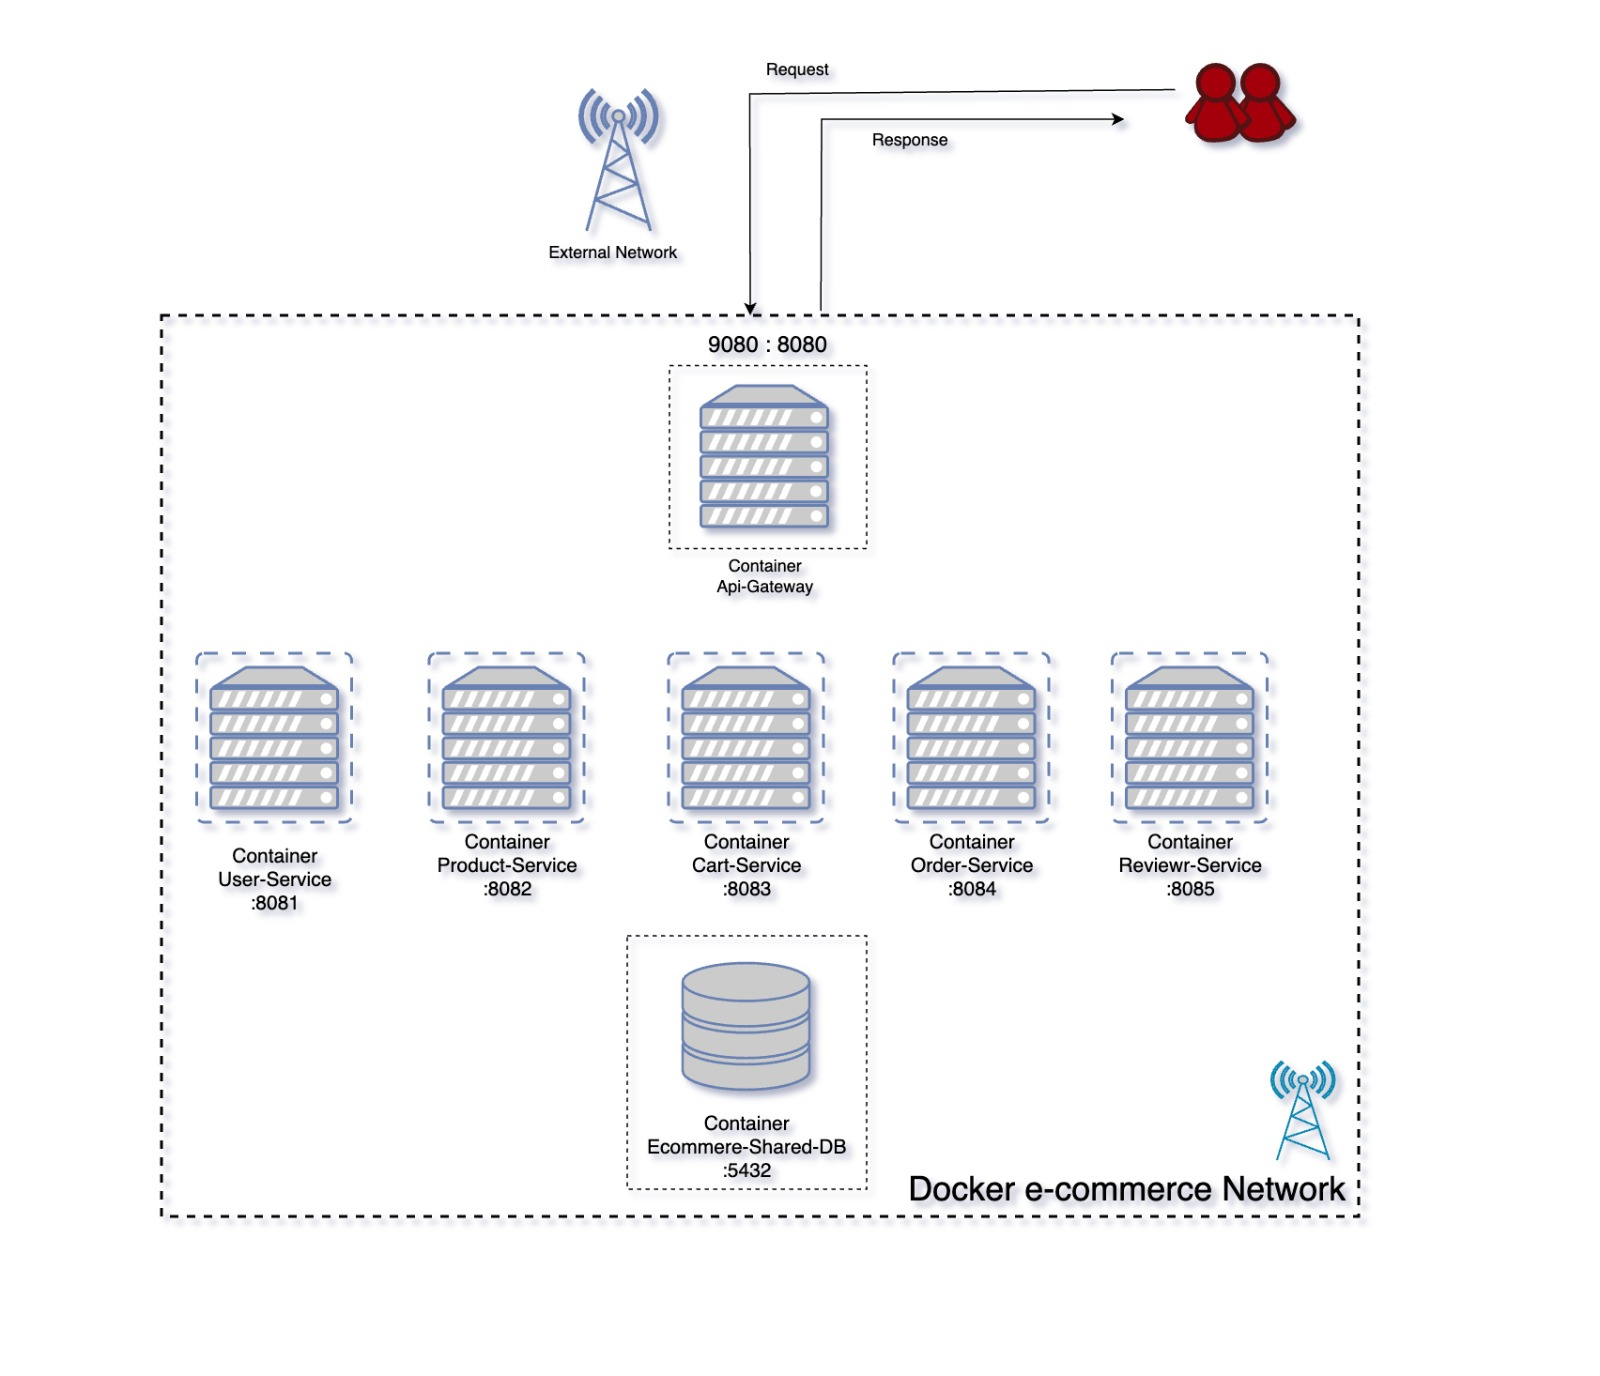
\includegraphics[width=0.95\textwidth]{images/arch-1.jpeg}
\caption{Architecture microservices de la plateforme e-commerce}
\label{fig:architecture-overview}
\end{figure}

La figure~\ref{fig:architecture-overview} illustre le flux de communication : les requêtes externes (External Network) arrivent à l'\textbf{API Gateway} (port 9080:8080) qui route vers les services backend appropriés. Chaque service communique avec la base de données partagée (\textbf{Ecommerce-Shared-DB}, port 5432) et expose ses propres APIs sur des ports dédiés :

\begin{itemize}
    \item \textbf{User-Service} (8081) : Gestion des utilisateurs et adresses
    \item \textbf{Product-Service} (8082) : Catalogue produits et catégories
    \item \textbf{Cart-Service} (8083) : Paniers d'achat utilisateur
    \item \textbf{Order-Service} (8084) : Commandes et leur cycle de vie
    \item \textbf{Review-Service} (8085) : Avis et évaluations produits
\end{itemize}

Tous les conteneurs appartiennent au réseau \texttt{Docker e-commerce Network}, permettant la résolution DNS automatique entre services.

\section{Points critiques pour le chaos engineering}

Cette architecture présente plusieurs caractéristiques qui en font une cible idéale pour les expérimentations de résilience :

\subsection{Single Point of Failure (SPOF)}

Chaque microservice est déployé en \textbf{instance unique} (pas de réplication), créant des SPOF potentiels. La défaillance d'un seul conteneur entraîne l'indisponibilité totale du service concerné.

\subsection{Dépendances inter-services}

Les services communiquent en mode \textbf{synchrone} via HTTP/REST (RestTemplate), sans mécanismes de résilience natifs :
\begin{itemize}
    \item Cart-Service dépend de User-Service et Product-Service
    \item Order-Service dépend de User-Service et Product-Service
    \item Review-Service dépend de User-Service et Product-Service
\end{itemize}

Une panne en cascade est donc possible : si Product-Service tombe, Cart-Service, Order-Service et Review-Service deviennent partiellement ou totalement inutilisables.

\subsection{Base de données partagée}

La base PostgreSQL représente un \textbf{SPOF critique} : tous les services y accèdent directement. Une défaillance ou une saturation de la base impacte l'ensemble du système.

\subsection{Réseau Docker bridge}

Le réseau \texttt{ecommerce-network} introduit une latence réseau variable et est susceptible aux perturbations (perte de paquets, délais, partitionnement réseau).

\section{Infrastructure d'observabilité}

Pour mesurer l'impact des fautes injectées, une stack complète de monitoring a été intégrée :

\subsection{Composants de monitoring}

\begin{itemize}
    \item \textbf{Prometheus} (port 9091) : Collecte des métriques en time-series avec scraping toutes les 15 secondes
    \item \textbf{Grafana} (port 3000) : Dashboards de visualisation et alerting
    \item \textbf{cAdvisor} (port 9092) : Métriques des conteneurs Docker (CPU, mémoire, réseau, I/O)
\end{itemize}

Cette infrastructure permettra de mesurer précisément l'impact des fautes : dégradation de latence, augmentation du taux d'erreurs, chute du débit, indisponibilité des services.

\section{Déploiement avec Docker Compose}

\subsection{Configuration de base}

Le fichier \texttt{docker-compose.yml} orchestre l'ensemble de l'infrastructure :

\begin{lstlisting}[language=YAML, caption={docker-compose.yml - Services principaux (extrait)}]
services:
  shared-postgres:
    image: postgres:15-alpine
    container_name: ecommerce-shared-postgres
    ports: ["5432:5432"]
    networks:
      - ecommerce-network

  user-service:
    build: ./user-service
    container_name: user-service
    ports: ["9081:8081"]
    depends_on: [shared-postgres]
    networks:
      - ecommerce-network

  product-service:
    build: ./product-service
    container_name: product-service
    ports: ["9082:8082"]
    depends_on: [shared-postgres]
    networks:
      - ecommerce-network

  # Cart, Order, Review services (similaire)
  
  api-gateway:
    build: ./api-gateway
    container_name: api-gateway
    ports: ["9080:8080"]
    environment:
      - SPRING_PROFILES_ACTIVE=docker
    depends_on:
      - user-service
      - product-service
      - cart-service
      - order-service
      - review-service
    networks:
      - ecommerce-network

networks:
  ecommerce-network:
    driver: bridge
\end{lstlisting}

\subsection{Configuration du monitoring}

\begin{lstlisting}[language=YAML, caption={docker-compose.yml - Stack d'observabilité (extrait)}]
  prometheus:
    image: prom/prometheus:latest
    container_name: prometheus
    ports: ["9091:9090"]
    volumes:
      - ./monitoring/prometheus.yml:/etc/prometheus/prometheus.yml
    networks:
      - ecommerce-network

  cadvisor:
    image: gcr.io/cadvisor/cadvisor:v0.47.0
    container_name: cadvisor
    ports: ["9092:8092"]
    volumes:
      - /:/rootfs:ro
      - /var/run:/var/run:ro
      - /sys:/sys:ro
      - /var/lib/docker/:/var/lib/docker:ro
    privileged: true
    command:
      - '--port=8092'
    networks:
      - ecommerce-network

  grafana:
    image: grafana/grafana:latest
    container_name: grafana
    ports: ["3000:3000"]
    environment:
      - GF_SECURITY_ADMIN_PASSWORD=admin
    networks:
      - ecommerce-network
\end{lstlisting}

\subsection{Configuration Prometheus}

\begin{lstlisting}[language=YAML, caption={monitoring/prometheus.yml - Cibles de scraping}]
global:
  scrape_interval: 15s

scrape_configs:
  # Métriques applicatives Spring Boot
  - job_name: 'spring-boot-apps'
    metrics_path: '/actuator/prometheus'
    static_configs:
      - targets:
          - 'user-service:8081'
          - 'product-service:8082'
          - 'cart-service:8083'
          - 'order-service:8084'
          - 'review-service:8085'
          - 'api-gateway:8080'

  # Métriques des conteneurs
  - job_name: 'cadvisor'
    static_configs:
      - targets: ['cadvisor:8092']
\end{lstlisting}

\section{Commandes de déploiement}

\begin{lstlisting}[caption={Démarrage de l'infrastructure complète}]
# Construction et démarrage de tous les services
docker compose up --build -d

# Vérification de l'état des conteneurs
docker compose ps

# Consultation des logs d'un service
docker compose logs -f product-service

# Arrêt et nettoyage complet
docker compose down -v
\end{lstlisting}

\subsection{Accès aux interfaces}

\begin{table}[H]
\centering
\begin{tabular}{ll}
\toprule
\textbf{Interface} & \textbf{URL} \\
\midrule
API Gateway & \texttt{http://localhost:9080} \\
Grafana & \texttt{http://localhost:3000} (admin/admin) \\
Prometheus & \texttt{http://localhost:9091} \\
cAdvisor & \texttt{http://localhost:9092} \\
Product Service (direct) & \texttt{http://localhost:9082} \\
\bottomrule
\end{tabular}
\caption{Points d'accès de l'infrastructure}
\end{table}

\section*{Conclusion du chapitre}

Ce chapitre a présenté l'architecture cible de nos expérimentations de chaos engineering : une plateforme e-commerce microservices avec cinq services métiers, une API Gateway et une base PostgreSQL partagée. 

Les caractéristiques clés identifiées sont :
\begin{itemize}
    \item \textbf{Instances uniques} : chaque service est un SPOF potentiel
    \item \textbf{Dépendances synchrones} : risque de pannes en cascade
    \item \textbf{Base partagée} : SPOF critique de données
    \item \textbf{Aucun mécanisme de résilience} : pas de retry, circuit breaker, timeout configuré
\end{itemize}

L'infrastructure de monitoring (Prometheus, Grafana, cAdvisor) est en place pour mesurer précisément l'impact des fautes qui seront injectées.

Dans le chapitre 2, nous présenterons les scénarios de test de charge et les protocoles d'injection de fautes qui seront appliqués sur cette architecture, en combinant JMeter pour générer la charge et Pumba pour injecter les pannes.